\documentclass[t,8pt]{beamer}
%\usetheme{boxes}
%\usecolortheme{default}

%%% packages
\geometry{paperwidth=140mm,paperheight=105mm}
\usefonttheme[onlymath]{serif}

\usepackage{kotex,amsmath,tabto,setspace,tikz}

\usepackage{xcolor}

%%% counters, commands, environments
\newcounter{num}
\resetcounteronoverlays{num}

\newenvironment{defi}[1]{\refstepcounter{num}\begin{block}{정의 \arabic{num}#1}}{\end{block}}
\newenvironment{theo}[1]{\refstepcounter{num}\begin{block}{정리 \arabic{num}#1}}{\end{block}}
\newenvironment{prob}[1]{\refstepcounter{num}\begin{block}{문제 \arabic{num}#1}}{\end{block}}
\newenvironment{exam}[1]{\refstepcounter{num}\begin{block}{예시 \arabic{num}#1}}{\end{block}}

\newcommand{\pb}[1]%\Phantom + fBox
{\fbox{\phantom{\ensuremath{#1}}}}
\newcommand{\rb}[2]%\Red+fBox
{\fbox{\uncover<#1>{\red{\ensuremath{#2}}}}}
\renewcommand{\arraystretch}{1.5}
\newcommand{\red}[1]{\color{red}{#1}}
\newcommand{\ivs}{\centering\strut\vspace*{-\baselineskip}\newline}%image vertical setting
\newcommand*\circled[1]{\tikz[baseline=(char.base)]{\node[shape=circle,draw,inner sep=2pt] (char) {#1};}}

%%% title
\title{수학 II : 01 함수의 극한과 연속}
\institute[ibedu]{김선중}
\date{\today}

%%% toc
\AtBeginSection[]
{\begin{frame}
    \frametitle{목차}
    \tableofcontents[currentsection]
  \end{frame}}


\begin{document}
%%
\frame{\titlepage}

%%%%
\section{함수의 극한}

%%%
\subsection{함수의 그래프}

%%
\begin{frame}[t]{\subsecname}
%
\begin{prob}{) 다음 함수의 그래프를 그리고 함숫값을 구하여라.}\:\par
\begin{minipage}[t]{.48\textwidth}
\centering
(1) \(f(x)=x+2\)\\[10pt]
\includegraphics<1>[width=.8\textwidth]{img/1-1-55}
\includegraphics<2>[width=.8\textwidth]{img/1-1-1}\\[10pt]
\[f(0)=\rb22\qquad f(2)=\rb24\]
\end{minipage}
\begin{minipage}[t]{.48\textwidth}
\centering
(2) \(f(x)=4-\frac12x\)\\[10pt]
\includegraphics<1>[width=.8\textwidth]{img/1-1-55}
\includegraphics<2>[width=.8\textwidth]{img/1-1-2}\\[10pt]
\[f(0)=\rb24\qquad f(2)=\rb23\]
\end{minipage}
\end{prob}
\end{frame}

%%
\begin{frame}[t]{\subsecname}
\addtocounter{num}{-1}
%
\begin{prob}{) 다음 함수의 그래프를 그리고 함숫값을 구하여라.}\:\par
\begin{minipage}[t]{.48\textwidth}
\centering
(3) \(f(x)=x^2+1\)\\[10pt]
\includegraphics<1>[width=.8\textwidth]{img/1-1-55}
\includegraphics<2>[width=.8\textwidth]{img/1-1-3}\\[10pt]
\[f(0)=\rb21\qquad f(1)=\rb22\]
\end{minipage}
\begin{minipage}[t]{.48\textwidth}
\centering
(4) \(f(x)=-x^2+3\)\\[10pt]
\includegraphics<1>[width=.8\textwidth]{img/1-1-55}
\includegraphics<2>[width=.8\textwidth]{img/1-1-4}\\[10pt]
\[f(0)=\rb23\qquad f(2)=\rb22\]
\end{minipage}
\end{prob}
\end{frame}

%%
\begin{frame}[t]{\subsecname}
\addtocounter{num}{-1}
%
\begin{prob}{) 다음 함수의 그래프를 그리고 함숫값을 구하여라.}\:\par
\begin{minipage}[t]{.48\textwidth}
\centering
(5) \(f(x)=\begin{cases}x&(x<2)\\x-3&(x\ge2)\end{cases}\)\\[10pt]
\includegraphics<1>[width=.8\textwidth]{img/1-1-55}
\includegraphics<2>[width=.8\textwidth]{img/1-1-5}\\[10pt]
\[f(0)=\rb20\qquad f(2)=\rb21\]
\end{minipage}
\begin{minipage}[t]{.48\textwidth}
\centering
(6) \(f(x)=\begin{cases}x^2&(x\le1)\\-x+3&(x>1)\end{cases}\)\\[10pt]
\includegraphics<1>[width=.8\textwidth]{img/1-1-55}
\includegraphics<2>[width=.8\textwidth]{img/1-1-6}\\[10pt]
\[f(1)=\rb21\qquad f(4)=\rb2{-1}\]
\end{minipage}
\end{prob}
\end{frame}

%%
\begin{frame}[t]{\subsecname}
\addtocounter{num}{-1}
%
\begin{prob}{) 다음 함수의 그래프를 그리고 함숫값을 구하여라.}\:\par
\begin{minipage}[t]{.48\textwidth}
\centering
(7) \(f(x)=|x|\)\\[10pt]
\includegraphics<1>[width=.8\textwidth]{img/1-1-55}
\includegraphics<2>[width=.8\textwidth]{img/1-1-7}\\[10pt]
\[f(-2)=\rb22\qquad f(0)=\rb20\]
\end{minipage}
\begin{minipage}[t]{.48\textwidth}
\centering
(8) \(f(x)=\frac{|x|}{x}\)\\[10pt]
\includegraphics<1>[width=.8\textwidth]{img/1-1-55}
\includegraphics<2>[width=.8\textwidth]{img/1-1-8}\\[10pt]
\[f(-2)=\rb2{-1}\qquad f(0)=\rb2\times\]
\end{minipage}
\end{prob}
\end{frame}

%%
\begin{frame}[t]{\subsecname}
\addtocounter{num}{-1}
%
\begin{prob}{) 다음 함수의 그래프를 그리고 함숫값을 구하여라.}\:\par
\begin{minipage}[t]{.48\textwidth}
\centering
(9) \(f(x)=\frac1x\)\\[10pt]
\includegraphics<1>[width=.8\textwidth]{img/1-1-55}
\includegraphics<2>[width=.8\textwidth]{img/1-1-9}\\[10pt]
\[f(1)=\rb21\qquad f(3)=\rb2{\frac13}\]
\[f(0)=\rb2\times\qquad f(-2)=\rb2{-\frac12}\]
\end{minipage}
\begin{minipage}[t]{.48\textwidth}
\centering
(10) \(f(x)=\sqrt x\)\\[10pt]
\includegraphics<1>[width=.8\textwidth]{img/1-1-55}
\includegraphics<2>[width=.8\textwidth]{img/1-1-10}\\[10pt]
\[f(1)=\rb21\qquad f(2)=\rb2{\sqrt2}\]
\[f(4)=\rb22\qquad f(0)=\rb20\]
\[f(-1)=\rb2\times\]
\end{minipage}
\end{prob}
\end{frame}

%%%
\subsection{좌극한과 우극한}

%%
\begin{frame}[t]{\subsecname}
%
\begin{prob}{) 다음 함수의 좌극한과 우극한을 계산하여라.}\:\par
\begin{minipage}[t]{.48\textwidth}
\centering
(1) \(f(x)=x+2\)\\[10pt]
\includegraphics<1>[width=.8\textwidth]{img/1-1-55}
\includegraphics<2>[width=.8\textwidth]{img/1-1-1}
\[\lim_{x\to2-}f(x)=\rb24\qquad\lim_{x\to2+}f(x)=\rb24\]
\end{minipage}
\begin{minipage}[t]{.48\textwidth}
\centering
(2) \(f(x)=4-\frac12x\)\\[10pt]
\includegraphics<1>[width=.8\textwidth]{img/1-1-55}
\includegraphics<2>[width=.8\textwidth]{img/1-1-2}
\[\lim_{x\to2-}f(x)=\rb23\qquad\lim_{x\to2+}f(x)=\rb23\]
\end{minipage}
\end{prob}
\end{frame}

%%
\begin{frame}[t]{\subsecname}
\addtocounter{num}{-1}
%
\begin{prob}{) 다음 함수의 좌극한과 우극한을 계산하여라.}\:\par
\begin{minipage}[t]{.48\textwidth}
\centering
(3) \(f(x)=x^2+1\)\\[10pt]
\includegraphics<1>[width=.8\textwidth]{img/1-1-55}
\includegraphics<2>[width=.8\textwidth]{img/1-1-3}
\[\lim_{x\to-1-}f(x)=\rb22\qquad\lim_{x\to-1+}f(x)=\rb22\]
\end{minipage}
\begin{minipage}[t]{.48\textwidth}
\centering
(4) \(f(x)=-x^2+3\)\\[10pt]
\includegraphics<1>[width=.8\textwidth]{img/1-1-55}
\includegraphics<2>[width=.8\textwidth]{img/1-1-4}
\[\lim_{x\to0-}f(x)=\rb23\qquad\lim_{x\to0+}f(x)=\rb23\]
\end{minipage}
\end{prob}
\end{frame}

%%
\begin{frame}[t]{\subsecname}
\addtocounter{num}{-1}
%
\begin{prob}{) 다음 함수의 좌극한과 우극한을 계산하여라.}\:\par
\begin{minipage}[t]{.48\textwidth}
\centering
(5) \(f(x)=\begin{cases}x&(x<2)\\x-3&(x\ge2)\end{cases}\)\\[10pt]
\includegraphics<1>[width=.8\textwidth]{img/1-1-55}
\includegraphics<2>[width=.8\textwidth]{img/1-1-5}
\[\lim_{x\to0-}f(x)=\rb20\qquad\lim_{x\to0+}f(x)=\rb20\]
\[\lim_{x\to2-}f(x)=\rb22\qquad\lim_{x\to2+}f(x)=\rb2{-1}\]
\end{minipage}
\begin{minipage}[t]{.48\textwidth}
\centering
(6) \(f(x)=\begin{cases}x^2&(x\le1)\\-x+3&(x>1)\end{cases}\)\\[10pt]
\includegraphics<1>[width=.8\textwidth]{img/1-1-55}
\includegraphics<2>[width=.8\textwidth]{img/1-1-6}
\[\lim_{x\to-1-}f(x)=\rb21\qquad\lim_{x\to-1+}f(x)=\rb21\]
\[\lim_{x\to1-}f(x)=\rb21\qquad\lim_{x\to1+}f(x)=\rb22\]
\end{minipage}
\end{prob}
\end{frame}

%%
\begin{frame}[t]{\subsecname}
\addtocounter{num}{-1}
%
\begin{prob}{) 다음 함수의 좌극한과 우극한을 계산하여라.}\:\par
\begin{minipage}[t]{.48\textwidth}
\centering
(7) \(f(x)=|x|\)\\[10pt]
\includegraphics<1>[width=.8\textwidth]{img/1-1-55}
\includegraphics<2>[width=.8\textwidth]{img/1-1-7}
\[\lim_{x\to0-}f(x)=\rb20\qquad\lim_{x\to0+}f(x)=\rb20\]
\[\lim_{x\to2-}f(x)=\rb22\qquad\lim_{x\to2+}f(x)=\rb22\]
\end{minipage}
\begin{minipage}[t]{.48\textwidth}
\centering
(8) \(f(x)=\frac{|x|}{x}\)\\[10pt]
\includegraphics<1>[width=.8\textwidth]{img/1-1-55}
\includegraphics<2>[width=.8\textwidth]{img/1-1-8}
\[\lim_{x\to-2-}f(x)=\rb2{-1}\qquad\lim_{x\to-2+}f(x)=\rb2{-1}\]
\[\lim_{x\to0-}f(x)=\rb2{-1}\qquad\lim_{x\to0+}f(x)=\rb21\]
\end{minipage}
\end{prob}
\end{frame}

%%
\begin{frame}[t]{\subsecname}
\addtocounter{num}{-1}
%
\begin{prob}{) 다음 함수의 좌극한과 우극한을 계산하여라.}\:\par
\begin{minipage}[t]{.48\textwidth}
\centering
(9) \(f(x)=\frac1x\)\\[10pt]
\includegraphics<1>[width=.8\textwidth]{img/1-1-55}
\includegraphics<2>[width=.8\textwidth]{img/1-1-9}\\[10pt]
\[\lim_{x\to1-}f(x)=\rb21\qquad\lim_{x\to1+}f(x)=\rb21\]
\[\lim_{x\to0-}f(x)=\rb2{-\infty}\qquad\lim_{x\to0+}f(x)=\rb2\infty\]
\end{minipage}
\begin{minipage}[t]{.48\textwidth}
\centering
(10) \(f(x)=\sqrt x\)\\[10pt]
\includegraphics<1>[width=.8\textwidth]{img/1-1-55}
\includegraphics<2>[width=.8\textwidth]{img/1-1-10}\\[10pt]
\[\lim_{x\to1-}f(x)=\rb21\qquad\lim_{x\to1+}f(x)=\rb21\]
\[\lim_{x\to0-}f(x)=\rb2\times\qquad\lim_{x\to0+}f(x)=\rb20\]
\end{minipage}
\end{prob}
\end{frame}

%%%
\subsection{함수의 극한}

%%
\begin{frame}[t]{\subsecname}
%
\begin{prob}{) 다음 함수의 극한값을 계산하여라.}\:\par
\begin{minipage}[t]{.48\textwidth}
\centering
(1) \(f(x)=x+2\)\\[10pt]
\includegraphics<1>[width=.8\textwidth]{img/1-1-55}
\includegraphics<2>[width=.8\textwidth]{img/1-1-1}
\[\lim_{x\to2-}f(x)=\rb24\qquad\lim_{x\to2+}f(x)=\rb24\]
\[\lim_{x\to2}f(x)=\rb24\]
\end{minipage}
\begin{minipage}[t]{.48\textwidth}
\centering
(2) \(f(x)=4-\frac12x\)\\[10pt]
\includegraphics<1>[width=.8\textwidth]{img/1-1-55}
\includegraphics<2>[width=.8\textwidth]{img/1-1-2}
\[\lim_{x\to2-}f(x)=\rb23\qquad\lim_{x\to2+}f(x)=\rb23\]
\[\lim_{x\to2}f(x)=\rb23\]
\end{minipage}
\end{prob}
\end{frame}

%%
\begin{frame}[t]{\subsecname}
\addtocounter{num}{-1}
%
\begin{prob}{) 다음 함수의 극한값을 계산하여라.}\:\par
\begin{minipage}[t]{.48\textwidth}
\centering
(3) \(f(x)=x^2+1\)\\[10pt]
\includegraphics<1>[width=.8\textwidth]{img/1-1-55}
\includegraphics<2>[width=.8\textwidth]{img/1-1-3}
\[\lim_{x\to-1-}f(x)=\rb22\qquad\lim_{x\to-1+}f(x)=\rb22\]
\[\lim_{x\to-1}f(x)=\rb22\]
\end{minipage}
\begin{minipage}[t]{.48\textwidth}
\centering
(4) \(f(x)=-x^2+3\)\\[10pt]
\includegraphics<1>[width=.8\textwidth]{img/1-1-55}
\includegraphics<2>[width=.8\textwidth]{img/1-1-4}
\[\lim_{x\to0-}f(x)=\rb23\qquad\lim_{x\to0+}f(x)=\rb23\]
\[\lim_{x\to0}f(x)=\rb23\]
\end{minipage}
\end{prob}
\end{frame}

%%
\begin{frame}[t]{\subsecname}
\addtocounter{num}{-1}
%
\begin{prob}{) 다음 함수의 극한값을 계산하여라.}\:\par
\begin{minipage}[t]{.48\textwidth}
\centering
(5) \(f(x)=\begin{cases}x&(x<2)\\x-3&(x\ge2)\end{cases}\)\\[10pt]
\includegraphics<1>[width=.8\textwidth]{img/1-1-55}
\includegraphics<2>[width=.8\textwidth]{img/1-1-5}
\[\lim_{x\to2-}f(x)=\rb22\qquad\lim_{x\to2+}f(x)=\rb2{-1}\]
\[\lim_{x\to2}f(x)=\rb2\times\]
\end{minipage}
\begin{minipage}[t]{.48\textwidth}
\centering
(6) \(f(x)=\begin{cases}x^2&(x\le1)\\-x+3&(x>1)\end{cases}\)\\[10pt]
\includegraphics<1>[width=.8\textwidth]{img/1-1-55}
\includegraphics<2>[width=.8\textwidth]{img/1-1-6}
\[\lim_{x\to1-}f(x)=\rb21\qquad\lim_{x\to1+}f(x)=\rb22\]
\[\lim_{x\to1}f(x)=\rb2\times\]
\end{minipage}
\end{prob}
\end{frame}

%%
\begin{frame}[t]{\subsecname}
\addtocounter{num}{-1}
%
\begin{prob}{) 다음 함수의 극한값을 계산하여라.}\:\par
\begin{minipage}[t]{.48\textwidth}
\centering
(7) \(f(x)=|x|\)\\[10pt]
\includegraphics<1>[width=.8\textwidth]{img/1-1-55}
\includegraphics<2>[width=.8\textwidth]{img/1-1-7}
\[\lim_{x\to0-}f(x)=\rb20\qquad\lim_{x\to0+}f(x)=\rb20\]
\[\lim_{x\to0}f(x)=\rb20\]
\end{minipage}
\begin{minipage}[t]{.48\textwidth}
\centering
(8) \(f(x)=\frac{|x|}{x}\)\\[10pt]
\includegraphics<1>[width=.8\textwidth]{img/1-1-55}
\includegraphics<2>[width=.8\textwidth]{img/1-1-8}
\[\lim_{x\to0-}f(x)=\rb2{-1}\qquad\lim_{x\to0+}f(x)=\rb21\]
\[\lim_{x\to0}f(x)=\rb2\times\]
\end{minipage}
\end{prob}
\end{frame}

%%
\begin{frame}[t]{\subsecname}
\addtocounter{num}{-1}
%
\begin{prob}{) 다음 함수의 극한값을 계산하여라.}\:\par
\begin{minipage}[t]{.48\textwidth}
\centering
(9) \(f(x)=\frac1x\)\\[10pt]
\includegraphics<1>[width=.8\textwidth]{img/1-1-55}
\includegraphics<2>[width=.8\textwidth]{img/1-1-9}
\[\lim_{x\to0-}f(x)=\rb2{-\infty}\qquad\lim_{x\to0+}f(x)=\rb2\infty\]
\[\lim_{x\to0}f(x)=\rb2\times\]
\end{minipage}
\begin{minipage}[t]{.48\textwidth}
\centering
(10) \(f(x)=\sqrt x\)\\[10pt]
\includegraphics<1>[width=.8\textwidth]{img/1-1-55}
\includegraphics<2>[width=.8\textwidth]{img/1-1-10}
\[\lim_{x\to0-}f(x)=\rb2\times\qquad\lim_{x\to0+}f(x)=\rb20\]
\[\lim_{x\to0}f(x)=\rb2\times\]
\end{minipage}
\end{prob}
\end{frame}

%%
\begin{frame}[t]{\subsecname}
%
\begin{prob}{) 다음 극한값을 계산하여라.}\par
\begin{minipage}[t]{.48\textwidth}\centering
\includegraphics<1>[width=.55\textwidth]{img/1-3-33}
\includegraphics<2>[width=.55\textwidth]{img/1-3-1}\par\smallskip
(1) \(\displaystyle\lim_{x\to-1}(2x+3)=\rb21\)
\end{minipage}
\begin{minipage}[t]{.48\textwidth}\centering
\includegraphics<1>[width=.55\textwidth]{img/1-3-33}
\includegraphics<2>[width=.55\textwidth]{img/1-3-2}\par\smallskip
(2) \(\displaystyle\lim_{x\to1}(x^2-4x+2)=\rb2{-1}\)
\end{minipage}\par\bigskip
\begin{minipage}[t]{.48\textwidth}\centering
\includegraphics<1>[width=.55\textwidth]{img/1-3-33}
\includegraphics<2>[width=.55\textwidth]{img/1-3-3}\par\smallskip
(3) \(\displaystyle\lim_{x\to2}\frac{|x-1|}{x-1}=\rb2\times\)
\end{minipage}
\begin{minipage}[t]{.48\textwidth}\centering
\includegraphics<1>[width=.55\textwidth]{img/1-3-33}
\includegraphics<2>[width=.55\textwidth]{img/1-3-4}\par\smallskip
(4) \(\displaystyle\lim_{x\to0}\left(|x|-2\right)=\rb2{-2}\)
\end{minipage}
\end{prob}
\end{frame}

%%
\begin{frame}[t]{\subsecname}
\alert{좌극한}과 \alert{우극한}이 같으면 극한값이 존재한다.
\begin{itemize}
\item
좌극한이 존재하고 : \(\displaystyle \lim_{x\to a-}f(x)=L_1\)
\item
우극한이 존재하고 : \(\displaystyle \lim_{x\to a-}f(x)=L_2\)
\item
좌극한과 우극한이 같으면 : \(L_1=L_2=L\)
\end{itemize}
\:\par
극한값 \(\displaystyle\lim_{x\to a}f(x)\)이 존재하고, 그 값은 \(L\)이다.
\[\lim_{x\to a-}f(x)=L\]
\begin{minipage}{.6\textwidth}
\vspace{-30pt}
%
\begin{defi}{) 함수의 극한}
함수 \(f(x)\)에서 \(x\)의 값이 \(x\neq a\)을 만족시키면서 한없이 \(a\)에 가까워질 때, \(f(x)\)의 값이 일정한 값 \(L\)에 한없이 가까워지면 
\medskip
\begin{center}
\(x\)가 \(a\)에 가까워질 때, \(f(x)\)는 \(L\)에 \alert{수렴}한다.
\end{center}
\medskip\par
\noindent라고 말하고 기호로
\[\lim_{x\to a}f(x)=L\]
로 나타낸다.
이때 \(L\)을 \(f(x)\)의 \alert{극한값}이라고 부른다.
\end{defi}
\end{minipage}
\begin{minipage}{.35\textwidth}
\vspace{-30pt}
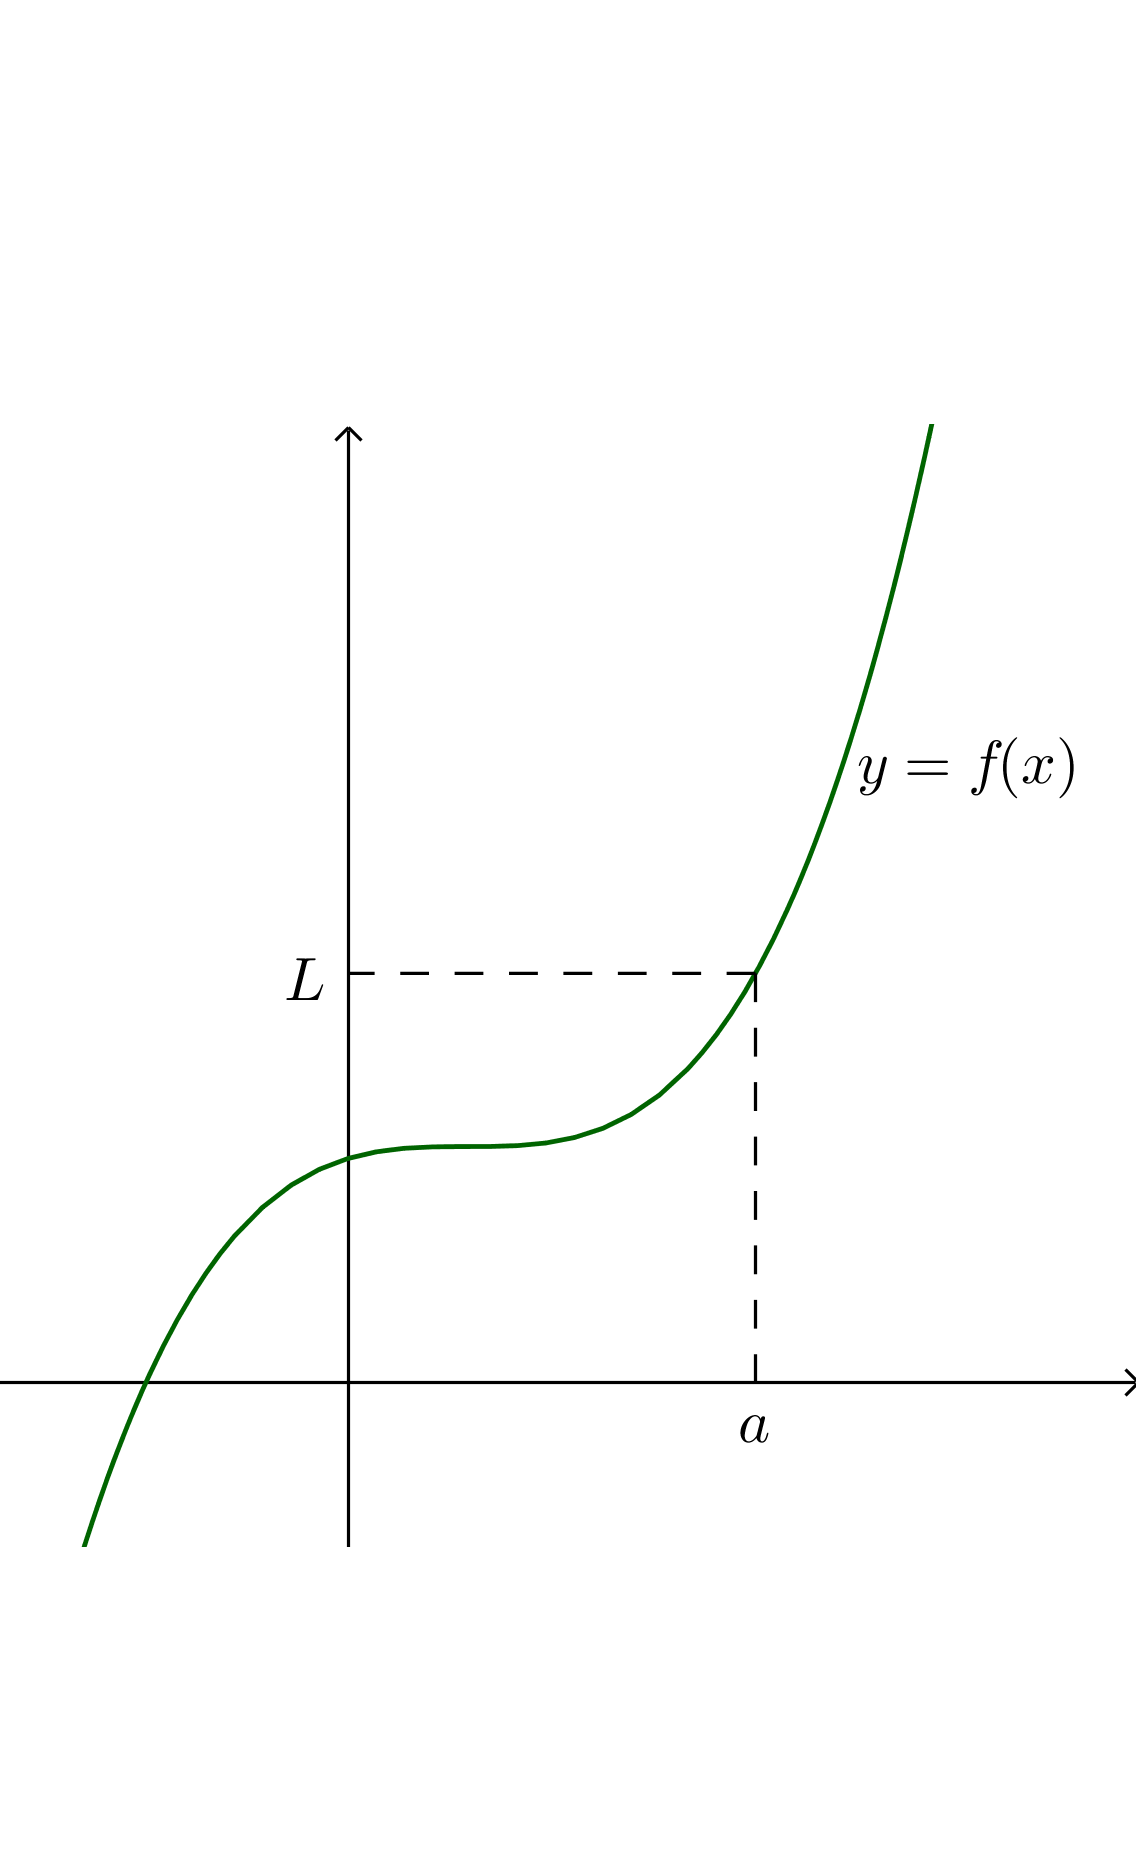
\includegraphics[width=\textwidth]{img/1-3-convergent_limit}
\end{minipage}
\end{frame}

%%%
\subsection{함수의 극한(무한대)}

%%
\begin{frame}[t]{\subsecname}
%
\begin{prob}{) 다음 함수의 극한을 조사하여라.}\:\par
\begin{minipage}[t]{.48\textwidth}
\centering
\includegraphics<1>[width=.8\textwidth]{img/1-4-55}
\includegraphics<2>[width=.8\textwidth]{img/1-4-1}
\[\lim_{x\to\infty}\left(\frac2x+1\right)=\rb21\]
\[\lim_{x\to-\infty}\left(\frac2x+1\right)=\rb21\]
\end{minipage}
\begin{minipage}[t]{.48\textwidth}
\centering
\includegraphics<1>[width=.8\textwidth]{img/1-4-55}
\includegraphics<2>[width=.8\textwidth]{img/1-4-2}
\[\lim_{x\to\infty}\left(\frac1{x-2}-1\right)=\rb2{-1}\]
\[\lim_{x\to-\infty}\left(\frac1{x-2}-1\right)=\rb2{-1}\]
\end{minipage}
\end{prob}
\end{frame}

%%
\begin{frame}[t]{\subsecname}
\addtocounter{num}{-1}
%
\begin{prob}{) 다음 함수의 극한을 조사하여라.}\:\par
\begin{minipage}[t]{.48\textwidth}
\centering
\includegraphics<1>[width=.8\textwidth]{img/1-4-55}
\includegraphics<2>[width=.8\textwidth]{img/1-4-3}
\[\lim_{x\to\infty}\frac1x=\rb20\]
\[\lim_{x\to-\infty}\frac1x=\rb20\]
\end{minipage}
\begin{minipage}[t]{.48\textwidth}
\centering
\includegraphics<1>[width=.8\textwidth]{img/1-4-55}
\includegraphics<2>[width=.8\textwidth]{img/1-4-4}
\[\lim_{x\to\infty}\left(\frac1{x-1}+2\right)=\rb22\]
\[\lim_{x\to-\infty}\left(\frac1{x-1}+2\right)=\rb22\]
\end{minipage}
\end{prob}
\end{frame}

%%
\begin{frame}[t]{\subsecname}
\addtocounter{num}{-1}
%
\begin{prob}{) 다음 함수의 극한을 조사하여라.}\:\par
\begin{minipage}[t]{.48\textwidth}
\centering
\includegraphics<1>[width=.8\textwidth]{img/1-4-55}
\includegraphics<2>[width=.8\textwidth]{img/1-4-5}
\[\lim_{x\to\infty}\left(x+2\right)=\rb2\infty\]
\[\lim_{x\to-\infty}\left(x+2\right)=\rb2{-\infty}\]
\end{minipage}
\begin{minipage}[t]{.48\textwidth}
\centering
\includegraphics<1>[width=.8\textwidth]{img/1-4-55}
\includegraphics<2>[width=.8\textwidth]{img/1-4-6}
\[\lim_{x\to\infty}x^2=\rb2\infty\]
\[\lim_{x\to-\infty}x^2=\rb2\infty\]
\end{minipage}
\end{prob}
\end{frame}

%%
\begin{frame}[t]{\subsecname}
\addtocounter{num}{-1}
%
\begin{prob}{) 다음 함수의 극한을 조사하여라.}\:\par
\begin{minipage}[t]{.48\textwidth}
\centering
\includegraphics<1>[width=.8\textwidth]{img/1-4-55}
\includegraphics<2>[width=.8\textwidth]{img/1-4-7}
\[\lim_{x\to\infty}\left(4-\frac12x\right)=\rb2{-\infty}\]
\[\lim_{x\to-\infty}\left(4-\frac12x\right)=\rb2\infty\]
\end{minipage}
\begin{minipage}[t]{.48\textwidth}
\centering
\includegraphics<1>[width=.8\textwidth]{img/1-4-55}
\includegraphics<2>[width=.8\textwidth]{img/1-4-8}
\[\lim_{x\to\infty}3=\rb23\]
\[\lim_{x\to-\infty}3=\rb23\]
\end{minipage}
\end{prob}
\end{frame}

%%%
\subsection{극한의 성질}

%%
\begin{frame}[t]{\subsecname(1)}
%
\begin{theo}{) 극한의 성질(1)}
두 극한 \(\displaystyle\lim_{x\to a}f(x)\)와 \(\displaystyle\lim_{x\to a}g(x)\)가 모두 수렴하면 다음 식이 성립한다.
\begin{enumerate}[(1)]
\item
\(\displaystyle\lim_{x\to a}kf(x)=k\lim_{x\to a}f(x)\)
\item
\(\displaystyle\lim_{x\to a}\left(f(x)+g(x)\right)=\lim_{x\to a}f(x)+\lim_{x\to a}g(x)\)
\item
\(\displaystyle\lim_{x\to a}\left(f(x)-g(x)\right)=\lim_{x\to a}f(x)-\lim_{x\to a}g(x)\)
\item
\(\displaystyle\lim_{x\to a}f(x)g(x)=\lim_{x\to a}f(x)\lim_{x\to a}g(x)\)
\item
\(\displaystyle\lim_{x\to a}\frac{f(x)}{g(x)}
=\frac{\displaystyle\lim_{x\to a}f(x)}{\displaystyle\lim_{x\to a}g(x)}\)
\end{enumerate}
\end{theo}
\uncover<2-3>{
%
\begin{prob}{}
\(\displaystyle\lim_{x\to a}f(x)=2\)와 \(\displaystyle\lim_{x\to a}g(x)=-5\)일 때, 다음 값들을 계산하시오.\par\;
\begin{enumerate}[(1)]
\setlength{\itemsep}{10pt}
\item
\(\displaystyle\lim_{x\to a}5f(x)\uncover<3>{=\red{10}}\)
\item
\(\displaystyle\lim_{x\to a}\left[f(x)+g(x)\right]\uncover<3>{=\red{-3}}\)
\item
\(\displaystyle\lim_{x\to a}\left[3f(x)+4g(x)\right]\uncover<3>{=\red{-14}}\)
\item
\(\displaystyle\lim_{x\to a}\left[3+2g(x)\right]\uncover<3>{=\red{-7}}\)
\end{enumerate}
\end{prob}}
\vspace{-120pt}
\uncover<4-5>{
%
\begin{prob}{) 다음 극한값을 계산하여라.}
\begin{enumerate}[(1)]
\setlength{\itemsep}{10pt}
\item
\(\displaystyle\lim_{x\to-1}(2x+3)\uncover<5>{=\red{1}}\)
\item
\(\displaystyle\lim_{x\to3}\left(x^2+x+3\right)\uncover<5>{=\red{15}}\)
\item
\(\displaystyle\lim_{x\to2}\frac{3x+2}{2x+1}\uncover<5>{=\red{\frac85}}\)
\item
\(\displaystyle\lim_{x\to1}(x^2+3)(x^2-4x+5)\uncover<5>{=\red{8}}\)
\end{enumerate}
\end{prob}}
\vspace{-120pt}
\uncover<6-7>{
\begin{minipage}{.6\textwidth}
%
\begin{prob}{) 다음 극한값을 계산하여라.}
\begin{enumerate}[(1)]
\setlength{\itemsep}{10pt}
\item
\(\displaystyle\lim_{x\to\infty}\frac{3x+5}{x+2}\uncover<7>{=\red3}\)
\item
\(\displaystyle\lim_{x\to\infty}\frac{x^2+3x+2}{2x^2-3x+1}\uncover<7>{=\red{\frac12}}\)
\item
\(\displaystyle\lim_{x\to\infty}\frac{2x+1}{x^2+x-2}\uncover<7>{=\red0}\)
\item
\(\displaystyle\lim_{x\to\infty}\frac{x^2-6x+3}{4x-2}\uncover<7>{=\red\infty}\)
\end{enumerate}
\end{prob}
\end{minipage}
\begin{minipage}[t]{.35\textwidth}
\vspace{-63pt}
\[\text{Hint : }\lim_{x\to\infty}\frac1x=0\]
\end{minipage}}
\end{frame}

%%
\begin{frame}[t]{\subsecname(2)}
%
\begin{theo}{) 극한의 성질(2)}
\[f(x)\le g(x)\quad\Longrightarrow\quad\lim_{x\to a}f(x)\le\lim_{x\to a}g(x)\]
\end{theo}
\uncover<2>{
%
\begin{exam}{}
\(x>0\)인 모든 실수 \(x\)에 대하여
\[4-x\le f(x)\le\frac4x\]
을 만족시킬 때, \(\displaystyle\lim_{x\to2}f(x)\)를 구하여라.

\bigskip
위의 식의 세 변에 모두 \(x\to2\)인 극한을 씌우면
\[\lim_{x\to 2}(4-x)\le\lim_{x\to 2}f(x)\le\lim_{x\to 2}\frac4x\]
\[2\le\lim_{x\to 2}f(x)\le2\]
이다.
따라서
\[\lim_{x\to 2}f(x)=2.\]
\end{exam}}
\vspace{-150pt}
\uncover<3-4>{
%
\begin{prob}{}
모든 실수 \(x\)에 대하여
\[4x-1\le f(x)\le x^2+3\]
을 만족시킬 때, \(\displaystyle\lim_{x\to2}f(x)\)를 구하여라.

\bigskip
위의 식의 세 변에 모두 \(x\to2\)인 극한을 씌우면
\[\rb4{\displaystyle\lim_{x\to 2}(4x-1)}\le\rb4{\displaystyle\lim_{x\to 2}f(x)}\le\rb4{\displaystyle\lim_{x\to 2}(x^2+3)}\]
\[\rb47\le\lim_{x\to 2}f(x)\le\rb47\]
이다.
따라서
\[\lim_{x\to 2}f(x)=\rb47.\]
\end{prob}}
\end{frame}

%%%%
\section{연속}

%%%
\subsection{한 점에서의 연속}

%%
\begin{frame}[t]{\subsecname}
\bigskip
\alert{함숫값}과 \alert{극한값}이 같으면 연속이다.
\begin{itemize}
\item
\(\text{함숫값}=f(a)\)
\item
\(\displaystyle\text{극한값}=\lim_{x\to a}f(x)\)
\end{itemize}
\par\bigskip
%
\begin{defi}{}\;\par
함수 \(f(x)\)와 실수 \(a\)에 대하여,
\[f(a)=\lim_{x\to a}f(x)\]
가 성립하면
\begin{center}\bfseries
함수 \(f(x)\)가 \(x=a\)에서 연속이다
\end{center}
라고 말한다.
\end{defi}
\end{frame}

%%
\begin{frame}[t]{\subsecname}
%
\begin{prob}{) 다음 함수의 연속성을 조사하여라.}\:\par
\begin{minipage}[t]{.48\textwidth}
\centering
(1) \(f(x)=x+2\)\\[10pt]
\includegraphics<1>[width=.8\textwidth]{img/1-1-55}
\includegraphics<2>[width=.8\textwidth]{img/1-1-1}
\[f(2)=\rb24\qquad\lim_{x\to2}f(x)=\rb24\]
\(f(x)\)는 \(x=2\)에서 ({\color<2>{red}{연속}}/불연속)이다.
\end{minipage}
\begin{minipage}[t]{.48\textwidth}
\centering
(2) \(f(x)=4-\frac12x\)\\[10pt]
\includegraphics<1>[width=.8\textwidth]{img/1-1-55}
\includegraphics<2>[width=.8\textwidth]{img/1-1-2}
\[f(2)=\rb24\qquad\lim_{x\to2}f(x)=\rb24\]
\(f(x)\)는 \(x=2\)에서 ({\color<2>{red}{연속}}/불연속)이다.
\end{minipage}
\end{prob}
\end{frame}

%%
\begin{frame}[t]{\subsecname}
\addtocounter{num}{-1}
%
\begin{prob}{) 다음 함수의 연속성을 조사하여라.}\:\par
\begin{minipage}[t]{.48\textwidth}
\centering
(3) \(f(x)=x^2+1\)\\[10pt]
\includegraphics<1>[width=.8\textwidth]{img/1-1-55}
\includegraphics<2>[width=.8\textwidth]{img/1-1-3}
\[f(-1)=\rb22\qquad\lim_{x\to-1}f(x)=\rb22\]
\(f(x)\)는 \(x=-1\)에서 ({\color<2>{red}{연속}}/불연속)이다.
\end{minipage}
\begin{minipage}[t]{.48\textwidth}
\centering
(4) \(f(x)=-x^2+3\)\\[10pt]
\includegraphics<1>[width=.8\textwidth]{img/1-1-55}
\includegraphics<2>[width=.8\textwidth]{img/1-1-4}
\[f(0)=\rb23\qquad\lim_{x\to0}f(x)=\rb23\]
\(f(x)\)는 \(x=0\)에서 ({\color<2>{red}{연속}}/불연속)이다.
\end{minipage}
\end{prob}
\end{frame}

%%
\begin{frame}[t]{\subsecname}
\addtocounter{num}{-1}
%
\begin{prob}{) 다음 함수의 연속성을 조사하여라.}\:\par
\begin{minipage}[t]{.48\textwidth}
\centering
(5) \(f(x)=\begin{cases}x&(x<2)\\x-3&(x\ge2)\end{cases}\)\\[10pt]
\includegraphics<1>[width=.8\textwidth]{img/1-1-55}
\includegraphics<2>[width=.8\textwidth]{img/1-1-5}
\[f(2)=\rb21\qquad\lim_{x\to2}f(x)=\rb2\times\]
\(f(x)\)는 \(x=0\)에서 (연속/{\color<2>{red}{불연속}})이다.
\end{minipage}
\begin{minipage}[t]{.48\textwidth}
\centering
(6) \(f(x)=\begin{cases}x^2&(x\le1)\\-x+3&(x>1)\end{cases}\)\\[10pt]
\includegraphics<1>[width=.8\textwidth]{img/1-1-55}
\includegraphics<2>[width=.8\textwidth]{img/1-1-6}
\[f(1)=\rb21\qquad\lim_{x\to1}f(x)=\rb2\times\]
\(f(x)\)는 \(x=1\)에서 (연속/{\color<2>{red}{불연속}})이다.
\end{minipage}
\end{prob}
\end{frame}

%%
\begin{frame}[t]{\subsecname}
\addtocounter{num}{-1}
%
\begin{prob}{) 다음 함수의 연속성을 조사하여라.}\:\par
\begin{minipage}[t]{.48\textwidth}
\centering
(7) \(f(x)=|x|\)\\[10pt]
\includegraphics<1>[width=.8\textwidth]{img/1-1-55}
\includegraphics<2>[width=.8\textwidth]{img/1-1-7}
\[f(0)=\rb20\qquad\lim_{x\to0}f(x)=\rb20\]
\(f(x)\)는 \(x=0\)에서 ({\color<2>{red}{연속}}/불연속)이다.
\end{minipage}
\begin{minipage}[t]{.48\textwidth}
\centering
(8) \(f(x)=\frac{|x|}{x}\)\\[10pt]
\includegraphics<1>[width=.8\textwidth]{img/1-1-55}
\includegraphics<2>[width=.8\textwidth]{img/1-1-8}
\[f(0)=\rb2\times\qquad\lim_{x\to2}f(x)=\rb2\times\]
\(f(x)\)는 \(x=0\)에서 (연속/{\color<2>{red}{불연속}})이다.
\end{minipage}
\end{prob}
\end{frame}

%%
\begin{frame}[t]{\subsecname}
\addtocounter{num}{-1}
%
\begin{prob}{) 다음 함수의 연속성을 조사하여라.}\:\par
\begin{minipage}[t]{.48\textwidth}
\centering
(9) \(f(x)=\frac1x\)\\[10pt]
\includegraphics<1>[width=.8\textwidth]{img/1-1-55}
\includegraphics<2>[width=.8\textwidth]{img/1-1-9}
\[f(0)=\rb2\times\qquad\lim_{x\to0}f(x)=\rb2\times\]
\(f(x)\)는 \(x=0\)에서 (연속/{\color<2>{red}{불연속}})이다.
\end{minipage}
\begin{minipage}[t]{.48\textwidth}
\centering
(10) \(f(x)=\sqrt x\)\\[10pt]
\includegraphics<1>[width=.8\textwidth]{img/1-1-55}
\includegraphics<2>[width=.8\textwidth]{img/1-1-10}
\[f(0)=\rb20\qquad\lim_{x\to0+}f(x)=\rb2\times\]
\(f(x)\)는 \(x=0\)에서 ({\color<2>{red}{연속}}/불연속)이다.
\end{minipage}
\end{prob}
\end{frame}

%%%
\subsection{구간}

%%
\begin{frame}[t]{\subsecname}
%
\begin{defi}{) 구간}
두 실수 \(a\), \(b\) (\(a<b\))에 대하여 다음과 같은 기호를 쓴다.
\begin{align*}
(a,b)&=\{x\;|\;a<x<b\}			\quad\cdots\cdots\quad\text{열린 구간}\\[5pt]
[a,b]&=\{x\;|\;a\le x\le b\}	\quad\cdots\cdots\quad\text{닫힌 구간}\\[5pt]
[a,b)&=\{x\;|\;a\le x<b\}\\[5pt]
(a,b]&=\{x\;|\;a<x\le b\}
\end{align*}
\end{defi}
%
\begin{prob}{) 다음 구간들을 그림으로 나타내어라.}
(1) \([1, 4]\)
\includegraphics<1>[width=\textwidth]{img/2-1-0}
\includegraphics<2>[width=\textwidth]{img/2-1-1}
\par\medskip
(2) \((-1, 3)\)
\includegraphics<1>[width=\textwidth]{img/2-1-0}
\includegraphics<2>[width=\textwidth]{img/2-1-2}
\par\medskip
(3) \((2, 5]\)
\includegraphics<1>[width=\textwidth]{img/2-1-0}
\includegraphics<2>[width=\textwidth]{img/2-1-3}
\end{prob}
\end{frame}

%%
\begin{frame}[t]{\subsecname}
\addtocounter{num}{-1}
%
\begin{prob}{) 다음 구간들을 그림으로 나타내어라.}
(4) \([-3, 2)\)
\includegraphics<1>[width=\textwidth]{img/2-1-0}
\includegraphics<2>[width=\textwidth]{img/2-1-4}
\par\medskip
(5) \((1, \infty)\)
\includegraphics<1>[width=\textwidth]{img/2-1-0}
\includegraphics<2>[width=\textwidth]{img/2-1-5}
\par\medskip
(6) \([-2, \infty)\)
\includegraphics<1>[width=\textwidth]{img/2-1-0}
\includegraphics<2>[width=\textwidth]{img/2-1-6}
\par\medskip
(7) \((-\infty,3)\)
\includegraphics<1>[width=\textwidth]{img/2-1-0}
\includegraphics<2>[width=\textwidth]{img/2-1-7}
\par\medskip
(8) \((-\infty,\infty)\)
\includegraphics<1>[width=\textwidth]{img/2-1-0}
\includegraphics<2>[width=\textwidth]{img/2-1-8}
\end{prob}
\end{frame}

%%%
\subsection{구간에서의 연속}

%%
\begin{frame}[t]{\subsecname}
%
\begin{prob}{) 다음 물음에 답하여라.}\:\par
\begin{minipage}[t]{.48\textwidth}
\centering
(1) \(f(x)=x+2\)\\[10pt]
\includegraphics<1>[width=.8\textwidth]{img/1-1-55}
\includegraphics<2>[width=.8\textwidth]{img/1-1-1}\par\medskip\raggedright
\quad\(f(x)\)는 \(x=2\)에서 ({\color<2>{red}{연속}}/불연속)이다.\par\medskip
\quad\(f(x)\)는 \(x=3\)에서 ({\color<2>{red}{연속}}/불연속)이다.\par\medskip
\quad\(f(x)\)는 \(x=4\)에서 ({\color<2>{red}{연속}}/불연속)이다.\par\medskip
\quad\(f(x)\)는 구간 \([2,4]\)에서 ({\color<2>{red}{연속}}/불연속)이다.
\end{minipage}
\begin{minipage}[t]{.48\textwidth}
\centering
(2) \(f(x)=4-\frac12x\)\\[10pt]
\includegraphics<1>[width=.8\textwidth]{img/1-1-55}
\includegraphics<2>[width=.8\textwidth]{img/1-1-2}\par\medskip\raggedright
\quad\(f(x)\)는 \(x=-2\)에서 ({\color<2>{red}{연속}}/불연속)이다.\par\medskip
\quad\(f(x)\)는 \(x=0\)에서 ({\color<2>{red}{연속}}/불연속)이다.\par\medskip
\quad\(f(x)\)는 \(x=2\)에서 ({\color<2>{red}{연속}}/불연속)이다.\par\medskip
\quad\(f(x)\)는 구간 \((-3,3)\)에서 ({\color<2>{red}{연속}}/불연속)이다.
\end{minipage}
\end{prob}
\end{frame}

%%
\begin{frame}[t]{\subsecname}
\addtocounter{num}{-1}
%
\begin{prob}{) 다음 함수의 극한값을 계산하여라.}\:\par
\begin{minipage}[t]{.48\textwidth}
\centering
(3) \(f(x)=x^2+1\)\\[10pt]
\includegraphics<1>[width=.8\textwidth]{img/1-1-55}
\includegraphics<2>[width=.8\textwidth]{img/1-1-3}\par\medskip\raggedright
\(f(x)\)는 구간 \((-\infty,\infty)\)에서 ({\color<2>{red}{연속}}/불연속)이다.
\end{minipage}
\begin{minipage}[t]{.48\textwidth}
\centering
(4) \(f(x)=-x^2+3\)\\[10pt]
\includegraphics<1>[width=.8\textwidth]{img/1-1-55}
\includegraphics<2>[width=.8\textwidth]{img/1-1-4}\par\medskip\raggedright
\(f(x)\)는 구간 \((-\infty,\infty)\)에서 ({\color<2>{red}{연속}}/불연속)이다.
\end{minipage}
\end{prob}
\end{frame}

%%
\begin{frame}[t]{\subsecname}
\addtocounter{num}{-1}
%
\begin{prob}{) 다음 함수의 극한값을 계산하여라.}\:\par
\begin{minipage}[t]{.48\textwidth}
\centering
(5) \(f(x)=\begin{cases}x&(x<2)\\x-3&(x\ge2)\end{cases}\)\\[10pt]
\includegraphics<1>[width=.8\textwidth]{img/1-1-55}
\includegraphics<2>[width=.8\textwidth]{img/1-1-5}\par\medskip\raggedright
\(f(x)\)는 구간 \((-\infty,1)\)에서 ({\color<2>{red}{연속}}/불연속)이다.\par\medskip
\(f(x)\)는 구간 \([0,3]\)에서 (연속/{\color<2>{red}{불연속}})이다.
\end{minipage}
\begin{minipage}[t]{.48\textwidth}
\centering
(6) \(f(x)=\begin{cases}x^2&(x\le1)\\-x+3&(x>1)\end{cases}\)\\[10pt]
\includegraphics<1>[width=.8\textwidth]{img/1-1-55}
\includegraphics<2>[width=.8\textwidth]{img/1-1-6}\par\medskip\raggedright
\(f(x)\)는 구간 \([0,2]\)에서 (연속/{\color<2>{red}{불연속}})이다.\par\medskip
\(f(x)\)는 구간 \([2,4]\)에서 ({\color<2>{red}{연속}}/불연속)이다.
\end{minipage}
\end{prob}
\end{frame}

%%
\begin{frame}[t]{\subsecname}
\addtocounter{num}{-1}
%
\begin{prob}{) 다음 함수의 극한값을 계산하여라.}\:\par
\begin{minipage}[t]{.48\textwidth}
\centering
(7) \(f(x)=|x|\)\\[10pt]
\includegraphics<1>[width=.8\textwidth]{img/1-1-55}
\includegraphics<2>[width=.8\textwidth]{img/1-1-7}\par\medskip\raggedright
\(f(x)\)는 구간 \(\rb2{(-\infty,\infty)}\)에서 연속이다.
\end{minipage}
\begin{minipage}[t]{.48\textwidth}
\centering
(8) \(f(x)=\frac{|x|}{x}\)\\[10pt]
\includegraphics<1>[width=.8\textwidth]{img/1-1-55}
\includegraphics<2>[width=.8\textwidth]{img/1-1-8}\par\medskip\raggedright
\(f(x)\)는 구간 \((-2,2)\)에서 (연속/{\color<2>{red}{불연속}})이다.\par\medskip
\(f(x)\)는 구간 \([2,\infty)\)에서 ({\color<2>{red}{연속}}/불연속)이다.
\end{minipage}
\end{prob}
\end{frame}

%%%
\subsection{연속함수의 성질}

%%
\begin{frame}[t]{\subsecname}
\begin{minipage}{.6\textwidth}
%
\begin{theo}{}\par\medskip\noindent
함수 \(f(x)\)와 \(g(x)\)가  \(x=a\)에서 연속이면\par\:
\begin{enumerate}[(1)]
\setlength{\itemsep}{13pt}
\item
\(kf(x)\)도 \(x=a\)에서 연속이다.
\item
\(f(x)+g(x)\)도 \(x=a\)에서 연속이다.
\item
\(f(x)-g(x)\)도 \(x=a\)에서 연속이다.
\item
\(f(x)g(x)\)도 \(x=a\)에서 연속이다.
\item
\(\displaystyle\frac{f(x)}{g(x)}\)도 \(x=a\)에서 연속이다. \quad(단, \(g(x)\neq0\))
\end{enumerate}
\end{theo}
\end{minipage}
%%
%\begin{prob}{}
%\begin{enumerate}[(1)]
%\setlength{\itemsep}{10pt}
%\item
%\(y=x^2+\frac1{x-2}\)는 \(x=0\)에서 (연속/{\color<2>{red}{불연속}})이다.
%\item
%\(y=x^2+\frac1{x-2}\)는 \(x=2\)에서 ({\color<2>{red}{연속}}/불연속)이다.
%\item
%\(y=\frac{x+2}{x^2-4}\)는 \(x=0\)에서 ({\color<2>{red}{연속}}/불연속)이다.
%\item
%\(y=\frac{x+2}{x^2-4}\)는 \(x=2\)에서 (연속/{\color<2>{red}{불연속}})이다.
%\end{enumerate}
%\end{prob}
\hspace{.05\textwidth}
\begin{minipage}[t]{.3\textwidth}
\centering
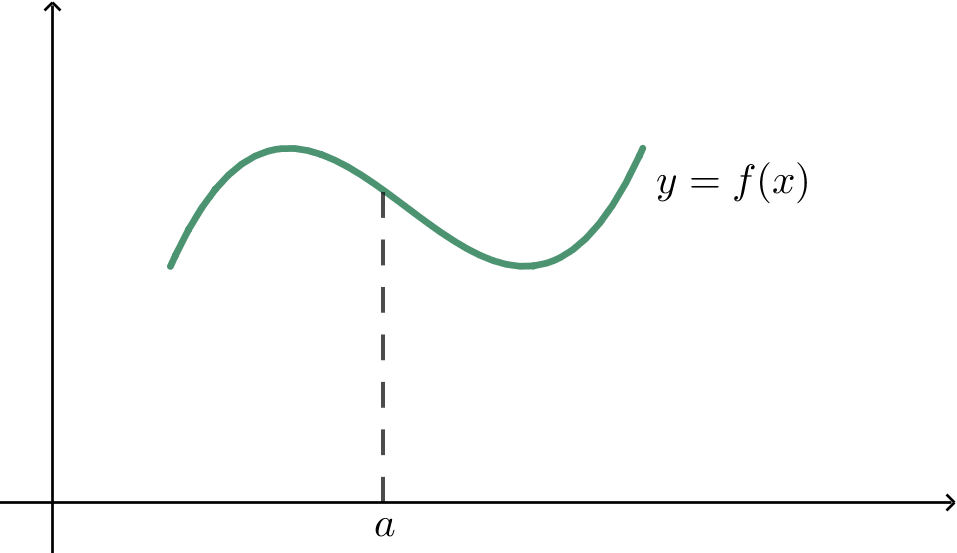
\includegraphics[width=\textwidth]{img/2-4-1}\\[10pt]
+\\[10pt]
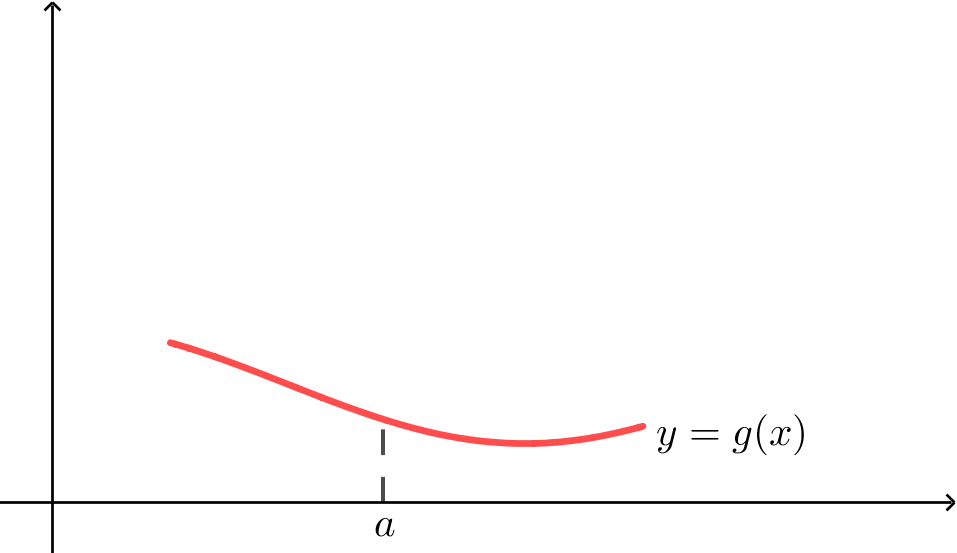
\includegraphics[width=\textwidth]{img/2-4-2}\\[10pt]
\(||\)\\[10pt]
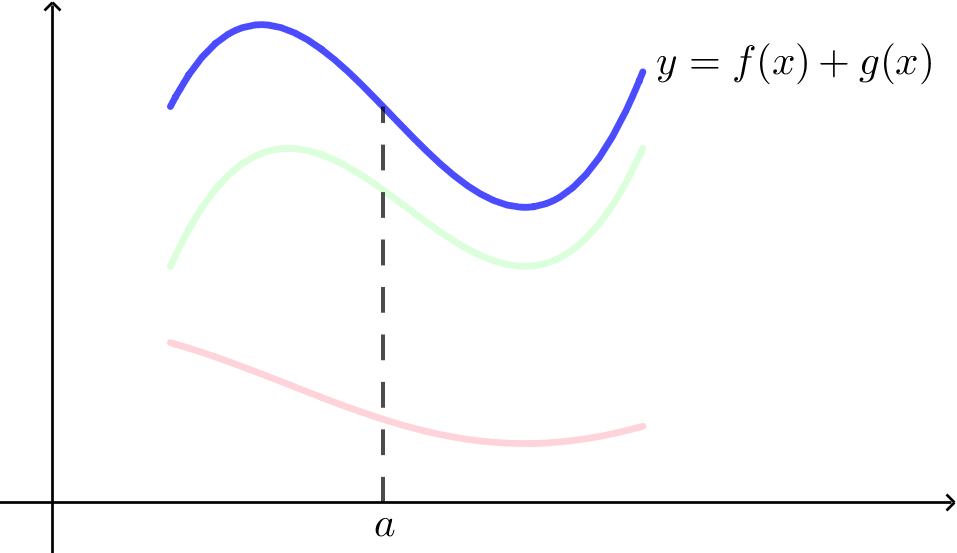
\includegraphics[width=\textwidth]{img/2-4-3}
\end{minipage}
\end{frame}

%%
\begin{frame}[t]{\subsecname}
\begin{prob}{}
\begin{enumerate}[(1)]
\setlength{\itemsep}{6pt}
\item
\(y=2x\)는 구간 \((-\infty,\infty)\)에서 ({\color<2>{red}{연속}}/불연속)이다.
\item
\(y=4\)는 구간 \((-\infty,\infty)\)에서 ({\color<2>{red}{연속}}/불연속)이다.
\item
\(y=2x-4\)는 구간 \((-\infty,\infty)\)에서 ({\color<2>{red}{연속}}/불연속)이다.
\item
\(y=x^2\)는 구간 \((-\infty,\infty)\)에서 ({\color<2>{red}{연속}}/불연속)이다.
\item
\(y=4x\)는 구간 \((-\infty,\infty)\)에서 ({\color<2>{red}{연속}}/불연속)이다.
\item
\(y=3\)는 구간 \((-\infty,\infty)\)에서 ({\color<2>{red}{연속}}/불연속)이다.
\item
\(y=x^2-4x+3\)는 구간 \((-\infty,\infty)\)에서 ({\color<2>{red}{연속}}/불연속)이다.
\item
\(y=\frac{x^2-4x+3}{2x-4}\)는 구간 \((-\infty,\infty)\)에서 (연속/{\color<2>{red}{불연속}})이다.
\item
\(y=\frac{x^2-4x+3}{2x-4}\)는 점 \(x=\rb22\)에서 불연속이다.
\item
\(y=\frac{x^2-4x+3}{2x-4}\)는 구간 \rb2{(-\infty,2)}, \rb2{(2,\infty)}에서 연속이다.
\item
\(y=\frac{2x-4}{x^2-4x+3}\)는 구간 \((-\infty,\infty)\)에서 (연속/{\color<2>{red}{불연속}})이다.
\item
\(y=\frac{2x-4}{x^2-4x+3}\)는 점 \(x=\rb21\), \(x=\rb23\)에서 불연속이다.
\item
\(y=\frac{2x-4}{x^2-4x+3}\)는 구간 \rb2{(-\infty,1)}, \rb2{(1,3)}, \rb2{(3,\infty)}에서 연속이다.
\end{enumerate}
\end{prob}
\end{frame}

%%%
%\begin{frame}[t]{\subsecname}
%\(f(x)\)가 \(x=a\)에서 연속이면 \(kf(x)\)도 \(x=a\)에서 연속이다.
%\end{frame}
%
%%%
%\begin{frame}[t]{\subsecname}
%\(f(x)\)와 \(g(x)\)가 \(x=a\)에서 연속이면 \(f(x)+g(x)\)도 \(x=a\)에서 연속이다.
%\end{frame}
%
%%%
%\begin{frame}[t]{\subsecname}
%\(f(x)\)와 \(g(x)\)가 \(x=a\)에서 연속이면 \(f(x)g(x)\)도 \(x=a\)에서 연속이다.
%\end{frame}


%%%
\subsection{최대\(\cdot\)최소의 정리}

%%
\begin{frame}[t]{\subsecname}
%
\begin{prob}{) 다음 함수들의 최댓값과 최솟값을 구하여라..}\par
\begin{minipage}[t]{.48\textwidth}\centering
\includegraphics<1>[width=.55\textwidth]{img/2-5-33}
\includegraphics<2>[width=.55\textwidth]{img/2-5-1}
\raisebox{40pt}{\begin{tabular}{cc}최댓값~:~\rb23\\최솟값~:~\rb2{-1}\end{tabular}}\par\smallskip
(1) \(y=x^2-1\quad[-1,2]\)
\end{minipage}
\begin{minipage}[t]{.48\textwidth}\centering
\includegraphics<1>[width=.55\textwidth]{img/2-5-33}
\includegraphics<2>[width=.55\textwidth]{img/2-5-2}
\raisebox{40pt}{\begin{tabular}{cc}최댓값~:~\rb2\times\\최솟값~:~\rb2{-1}\end{tabular}}\par\smallskip
(2) \(y=x^2-1\quad(-1,2)\)
\end{minipage}\par\bigskip
\begin{minipage}[t]{.48\textwidth}\centering
\includegraphics<1>[width=.55\textwidth]{img/2-5-33}
\includegraphics<2>[width=.55\textwidth]{img/2-5-3}
\raisebox{40pt}{\begin{tabular}{cc}최댓값~:~\rb23\\최솟값~:~\rb2{-3}\end{tabular}}\par\smallskip
(3) \(y=-2x+3\quad[0,3]\)
\end{minipage}
\begin{minipage}[t]{.48\textwidth}\centering
\includegraphics<1>[width=.55\textwidth]{img/2-5-33}
\includegraphics<2>[width=.55\textwidth]{img/2-5-4}
\raisebox{40pt}{\begin{tabular}{cc}최댓값~:~\rb2\times\\최솟값~:~\rb2\times\end{tabular}}\par\smallskip
(4) \(y=-2x+3\quad(0,3)\)
\end{minipage}
\end{prob}
\end{frame}

%%
\begin{frame}[t]{\subsecname}
%
\begin{prob}{) 다음 함수들의 최댓값과 최솟값을 구하여라..}\par
\begin{minipage}[t]{.48\textwidth}\centering
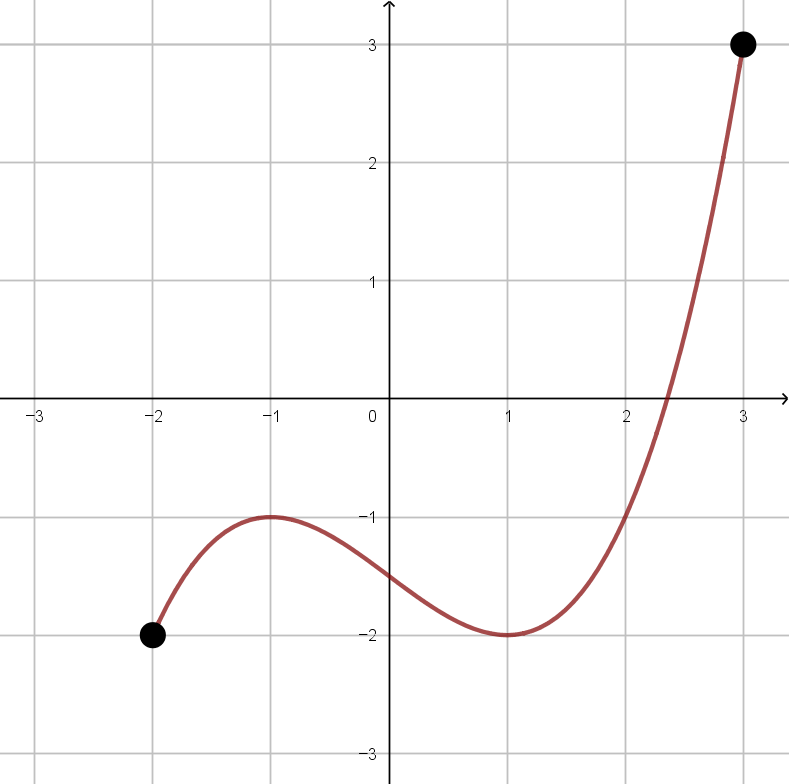
\includegraphics[width=.55\textwidth]{img/2-5-5}
\raisebox{40pt}{\begin{tabular}{cc}최댓값~:~\rb23\\최솟값~:~\rb2{-2}\end{tabular}}\par\smallskip
(5) \(y=\frac14\left(x^3-3x-6\right)\quad[-2,3]\)
\end{minipage}
\begin{minipage}[t]{.48\textwidth}\centering
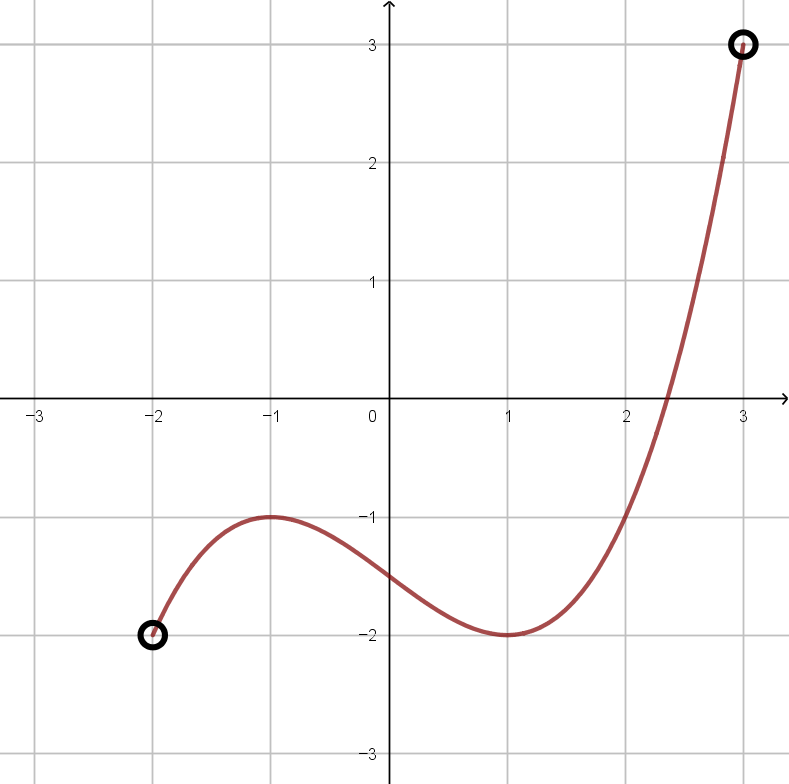
\includegraphics[width=.55\textwidth]{img/2-5-6}
\raisebox{40pt}{\begin{tabular}{cc}최댓값~:~\rb2\times\\최솟값~:~\rb2{-2}\end{tabular}}\par\smallskip
(6) \(y=\frac14\left(x^3-3x-6\right)\quad(-2,3)\)
\end{minipage}\par\bigskip
\begin{minipage}[t]{.48\textwidth}\centering
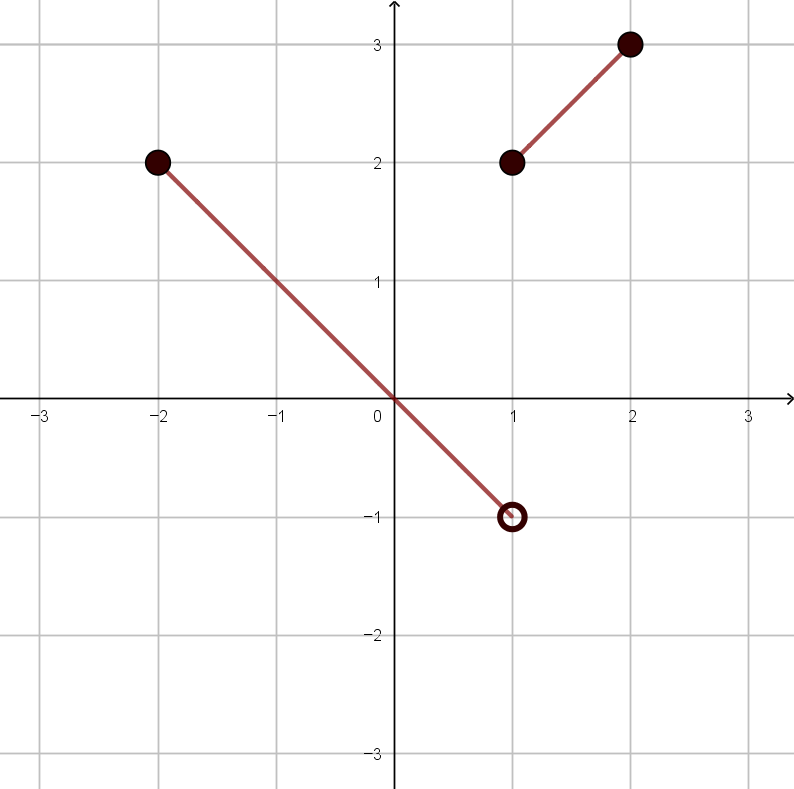
\includegraphics[width=.55\textwidth]{img/2-5-7}
\raisebox{40pt}{\begin{tabular}{cc}최댓값~:~\rb23\\최솟값~:~\rb2{\times}\end{tabular}}\par\smallskip
(7) \(y=\begin{cases}-x&(x<1)\\x+1&(x\ge1)\end{cases}\quad[-3,2]\)
\end{minipage}
\begin{minipage}[t]{.48\textwidth}\centering
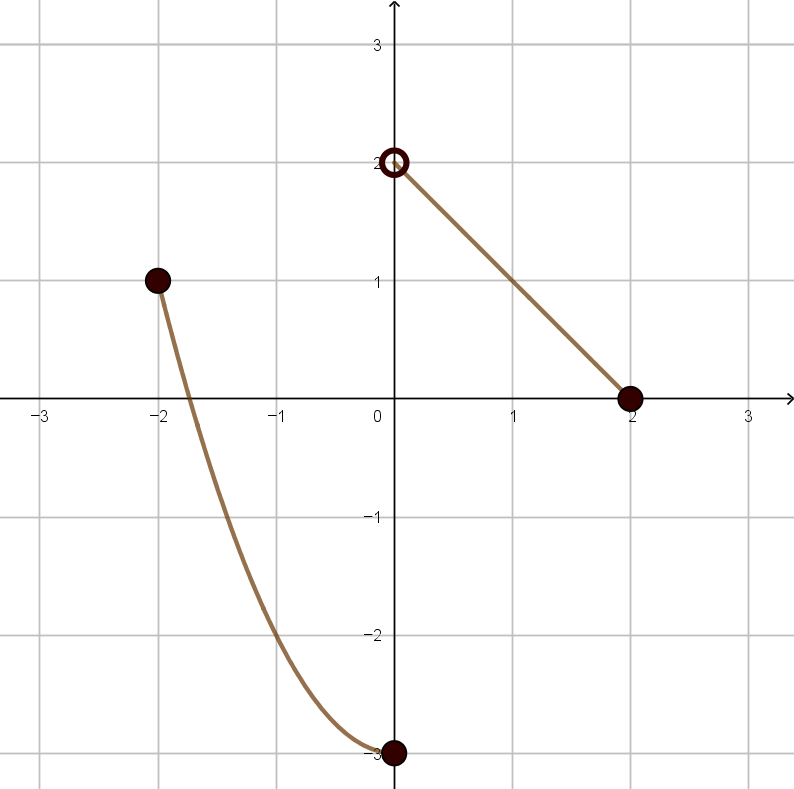
\includegraphics[width=.55\textwidth]{img/2-5-8}
\raisebox{40pt}{\begin{tabular}{cc}최댓값~:~\rb2\times\\최솟값~:~\rb2{-3}\end{tabular}}\par\smallskip
(8) \(y=\begin{cases}x^2-3&(x\le0)\\-x+2&(x>0)\end{cases}\quad[-2.2]\)
\end{minipage}
\end{prob}
\end{frame}
%%
\begin{frame}[t]{\subsecname}
%
\begin{theo}{) 최대·최소의 정리}
함수 \(f(x)\)가 \alert{닫힌 구간} \([a,b]\)에서 \alert{연속}이면, \(f(x)\)는 이 구간에서 최댓값과 최솟값을 가진다.
\end{theo}

\bigskip\bigskip
\uncover<2>{\begin{tabular}{ccc}
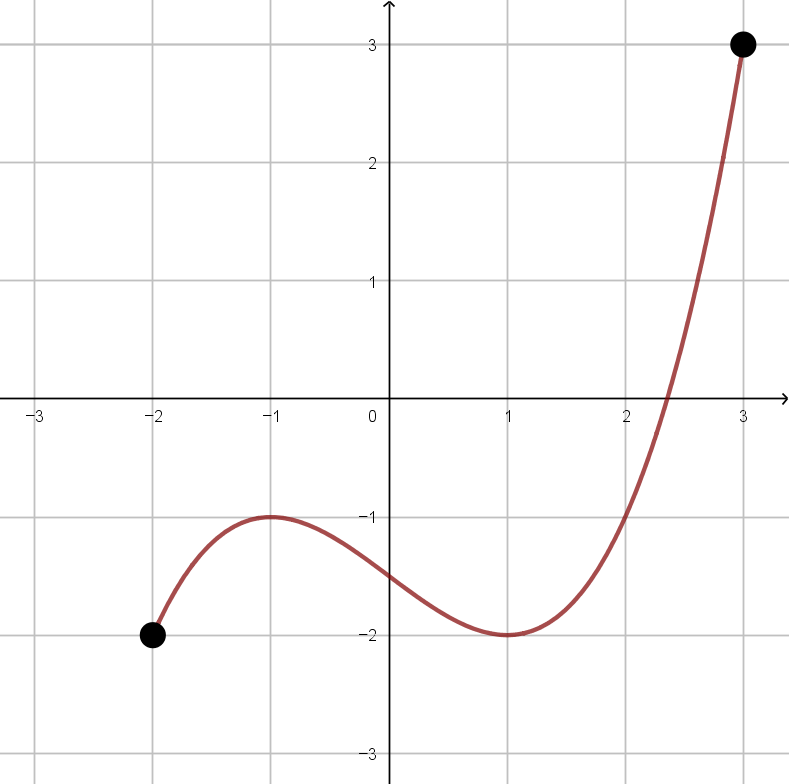
\includegraphics[width=.3\textwidth]{img/2-5-5}
&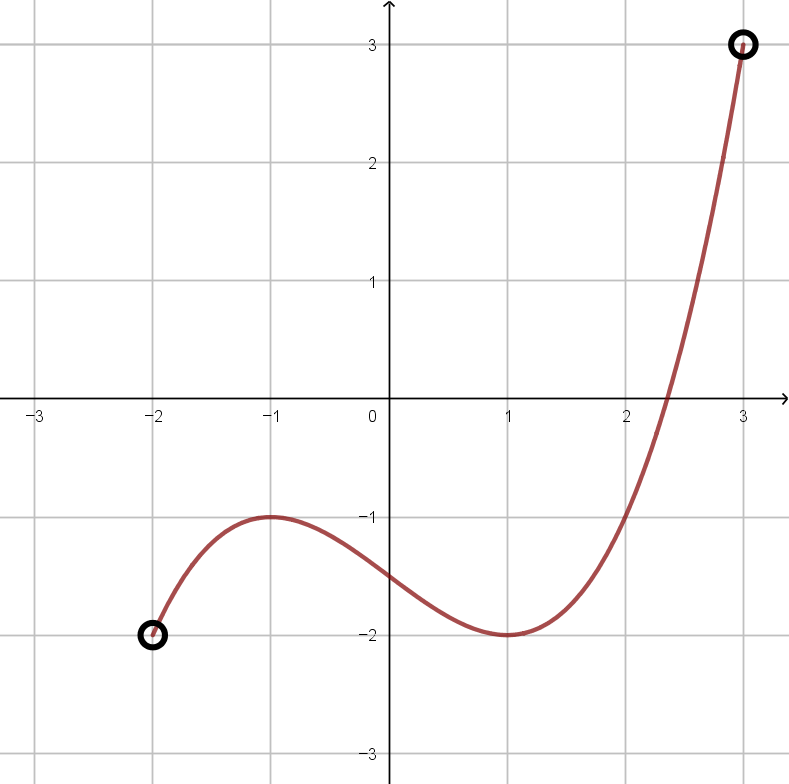
\includegraphics[width=.3\textwidth]{img/2-5-6}
&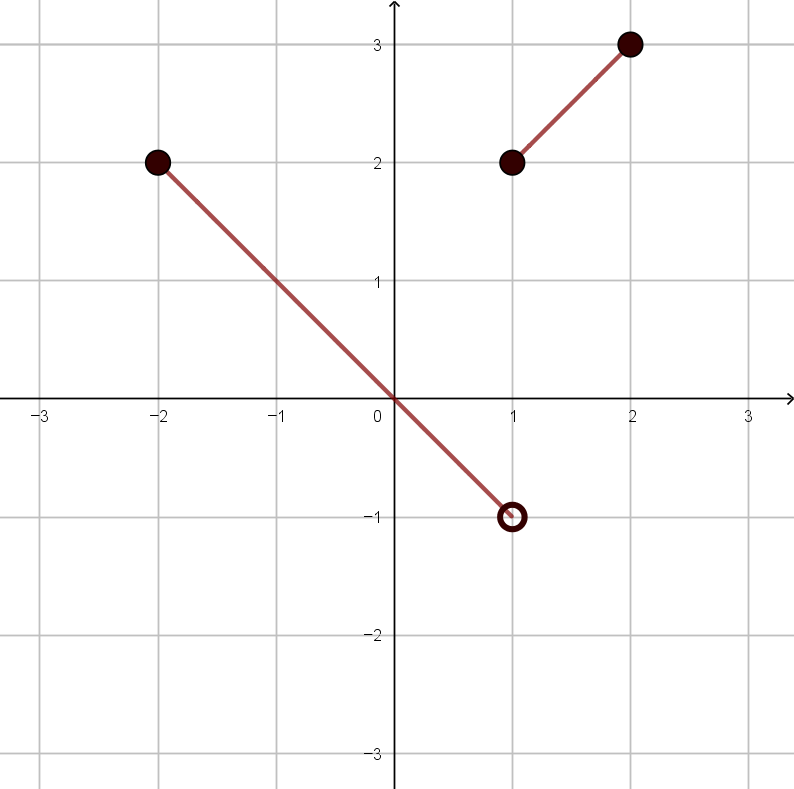
\includegraphics[width=.3\textwidth]{img/2-5-7}\\
닫힌구간			&열린구간		&닫힌구간\\
연속				&연속			&불연속\\
최대·최소 존재 O	&최대·최소 존재 X	&최대·최소 존재 X
\end{tabular}}

\end{frame}

%%%
\subsection{사잇값 정리}

%%
\begin{frame}[t]{\subsecname}
%
\begin{theo}{) 사잇값 정리}
함수 \(f(x)\)가 닫힌구간 \([a,b]\)에서 연속이고 \(f(a)<k<f(b)\)이면
\[f(c)=k\]
를 만족시키는 실수 \(c\)가 적어도 하나 존재한다. (단, \(a<c<b\))
\end{theo}

%
\begin{exam}{}
다음 그림은 \(a=1\), \(b=5\), \(f(a)=1\), \(f(b)=4\), \(k=3\)인 상황이다.\\
\begin{center}
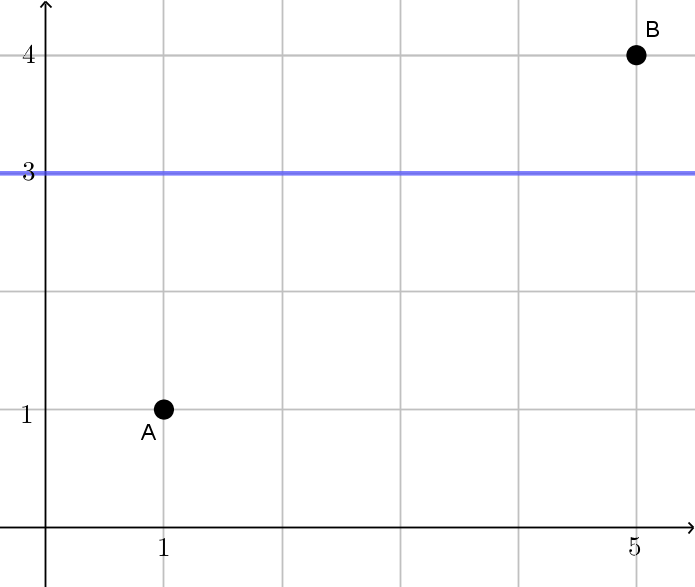
\includegraphics[width=.3\textwidth]{img/2-6-1-0}
\end{center}
\end{exam}
두 점 \(A(1,1)\), \(B(5,4)\)를 연속적으로 이어서 함수 \(y=f(x)\)를 만들고, 그때의 \(c\)값을 표시하여라.
\end{frame}

%%
\begin{frame}[t]{\subsecname}
두 점 \(A\)와 \(B\)를 연속적으로 이어서 \(y=f(x)\)의 그래프를 그리면, 반드시 파란 선 (\(y=3\))과 만난다.
이 만나는 점의 \(x\)좌표가 \(c\)의 값이 된다.
\begin{center}
%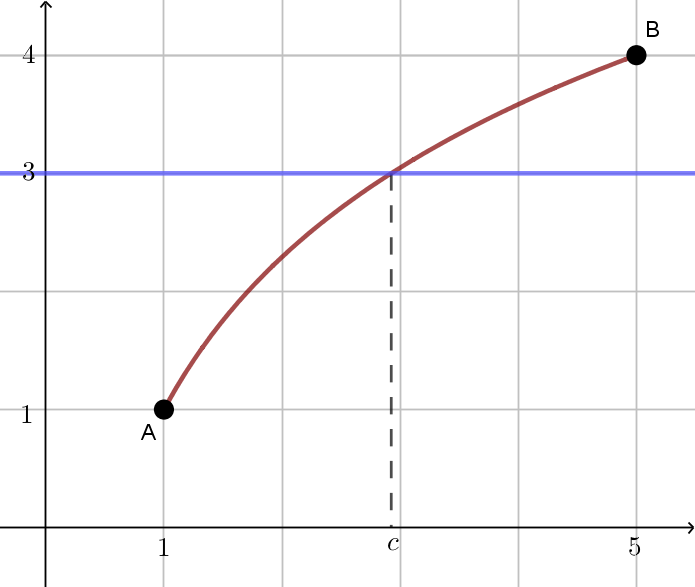
\includegraphics[width=.33\textwidth]{img/2-6-1-1}
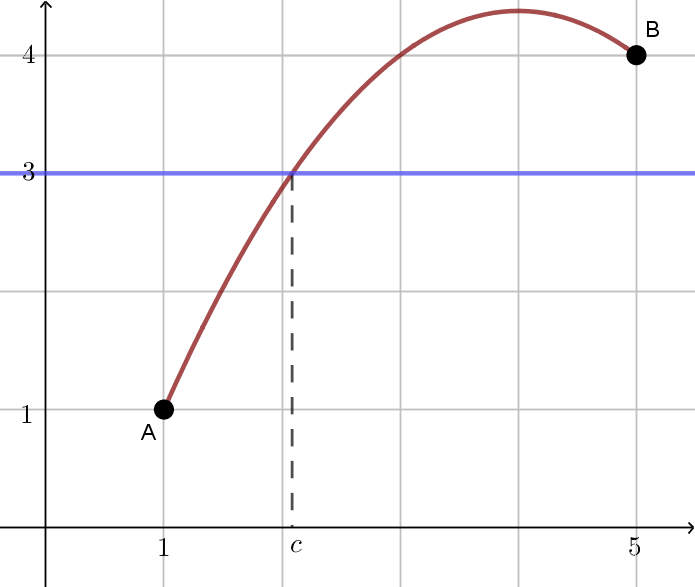
\includegraphics[width=.33\textwidth]{img/2-6-1-2}\qquad
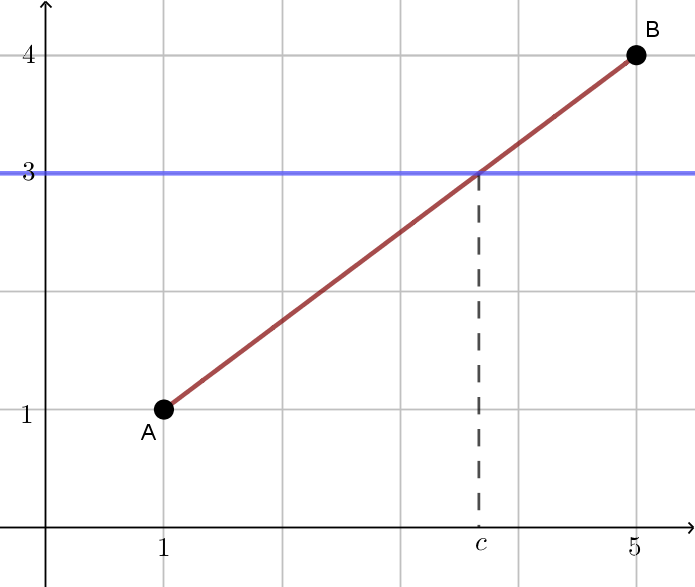
\includegraphics[width=.33\textwidth]{img/2-6-1-3}\\[20pt]
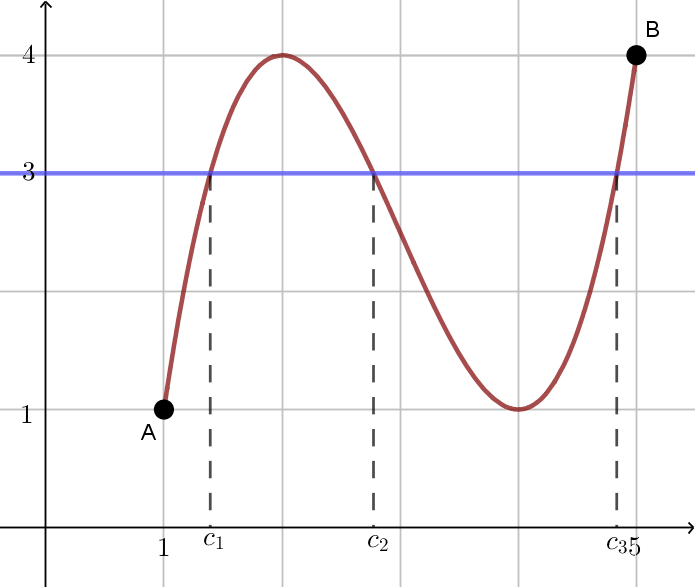
\includegraphics[width=.33\textwidth]{img/2-6-1-4}\qquad
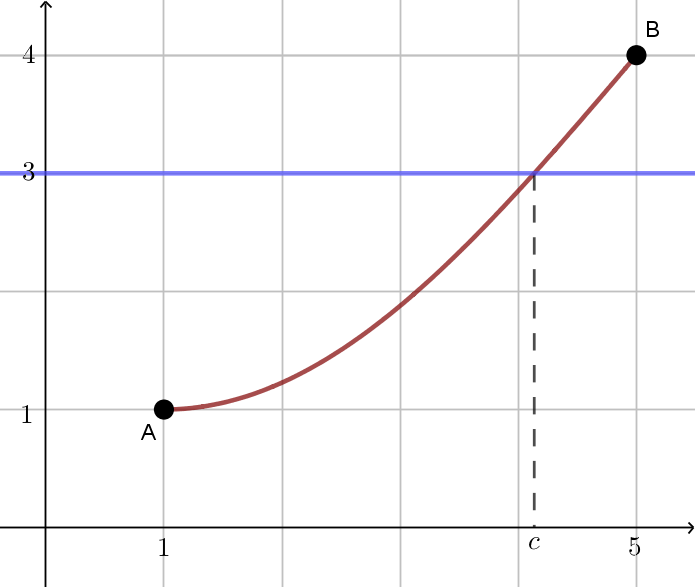
\includegraphics[width=.33\textwidth]{img/2-6-1-5}
\end{center}
\end{frame}

%%
\begin{frame}[t]{\subsecname}
\begin{minipage}{.6\textwidth}
\begin{prob}{}
실수 전체에서 연속인 함수 \(f(x)\)에 대하여\\[5pt]
\(f(2)=1\), \(f(3)=5\), \(f(5)=3\)일때,\\[5pt]
다음 중 옳은 것을 골라라.\\[5pt]
\begin{itemize}
\item[ㄱ.]
\(f(x)=2\)를 만족시키는 \(x\)가 적어도 하나 존재한다.
\item[ㄴ.]
\(f(x)=4\)를 만족시키는 \(x\)가 두 개 이상 존재한다.
\item[ㄷ.]
방정식 \(f(x)=-1\)의 해가 적어도 하나 존재한다.
\end{itemize}
\end{prob}
\end{minipage}
\begin{minipage}{.3\textwidth}
\begin{center}
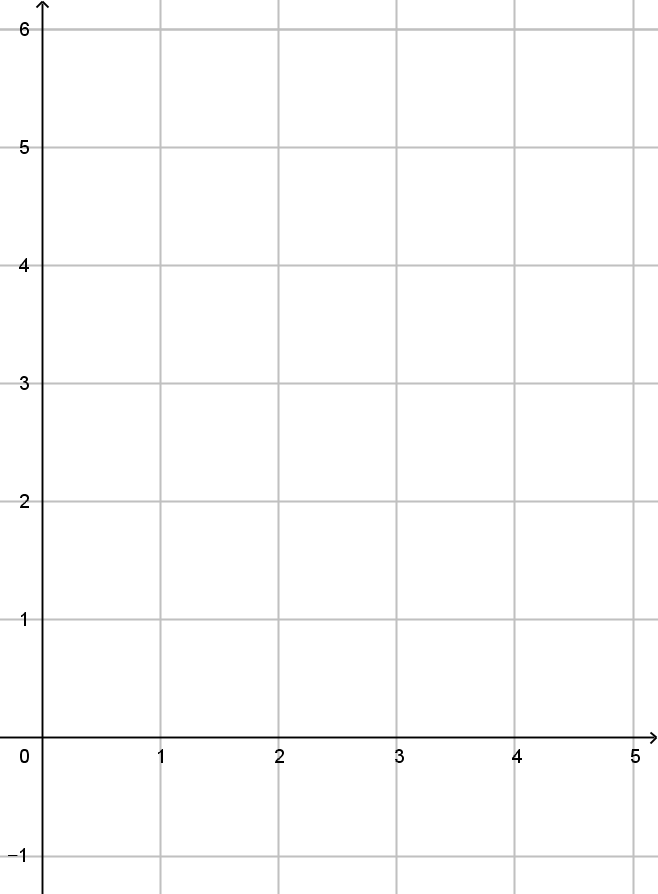
\includegraphics[width=.8\textwidth]{img/2-6-2-0}
\end{center}
\end{minipage}
\par\bigskip\bigskip
\begin{minipage}{.6\textwidth}
\begin{prob}{}
실수 전체에서 연속인 함수 \(f(x)\)에 대하여\\[5pt]
\(f(1)=3\), \(f(3)=-1\), \(f(5)=1\)일때,\\[5pt]
다음 중 옳은 것을 골라라.\\[5pt]
\begin{itemize}
\item[ㄱ.]
\(f(x)=2\)를 만족시키는 \(x\)가 적어도 하나 존재한다.
\item[ㄴ.]
\(f(x)=4\)를 만족시키는 \(x\)가 적어도 하나 존재한다.
\item[ㄷ.]
방정식 \(f(x)=0\)의 해가 적어도 두 개 이상 존재한다.
\end{itemize}
\end{prob}
\end{minipage}
\begin{minipage}{.3\textwidth}
\begin{center}
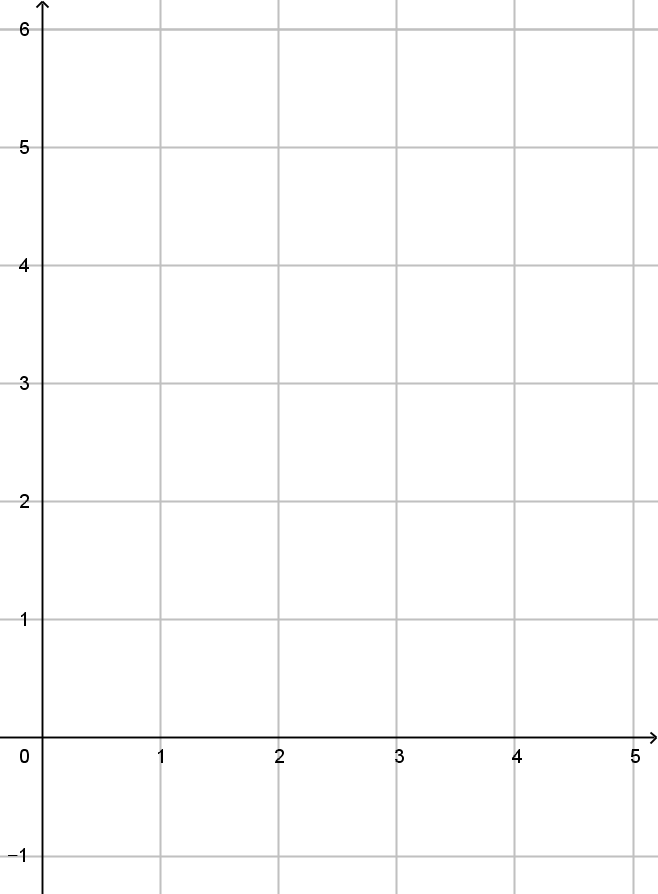
\includegraphics[width=.8\textwidth]{img/2-6-2-0}
\end{center}
\end{minipage}
\end{frame}

\addtocounter{num}{-2}
%%
\begin{frame}[t]{\subsecname}
\begin{minipage}{.6\textwidth}
\begin{prob}{}
실수 전체에서 연속인 함수 \(f(x)\)에 대하여\\[5pt]
\(f(2)=1\), \(f(3)=5\), \(f(5)=3\)일때,\\[5pt]
다음 중 옳은 것을 골라라.\\[5pt]
\begin{itemize}
\item[\textcircled{ㄱ}.]
\(f(x)=2\)를 만족시키는 \(x\)가 적어도 하나 존재한다.
\item[\textcircled{ㄴ}.]
\(f(x)=4\)를 만족시키는 \(x\)가 두 개 이상 존재한다.
\item[ㄷ.]
방정식 \(f(x)=-1\)의 해가 적어도 하나 존재한다.
\end{itemize}
\end{prob}
\end{minipage}
\begin{minipage}{.3\textwidth}
\begin{center}
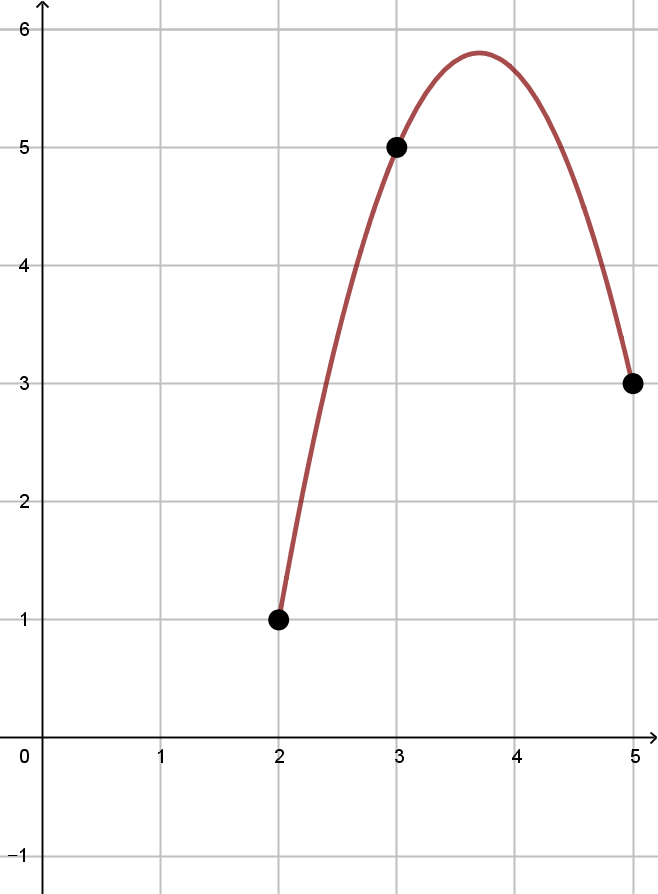
\includegraphics[width=.8\textwidth]{img/2-6-2-1}
\end{center}
\end{minipage}
\par\bigskip\bigskip
\begin{minipage}{.6\textwidth}
\begin{prob}{}
실수 전체에서 연속인 함수 \(f(x)\)에 대하여\\[5pt]
\(f(1)=3\), \(f(3)=-1\), \(f(5)=1\)일때,\\[5pt]
다음 중 옳은 것을 골라라.\\[5pt]
\begin{itemize}
\item[\textcircled{ㄱ}.]
\(f(x)=2\)를 만족시키는 \(x\)가 적어도 하나 존재한다.
\item[ㄴ.]
\(f(x)=4\)를 만족시키는 \(x\)가 적어도 하나 존재한다.
\item[\textcircled{ㄷ}.]
방정식 \(f(x)=0\)의 해가 적어도 두 개 이상 존재한다.
\end{itemize}
\end{prob}
\end{minipage}
\begin{minipage}{.3\textwidth}
\begin{center}
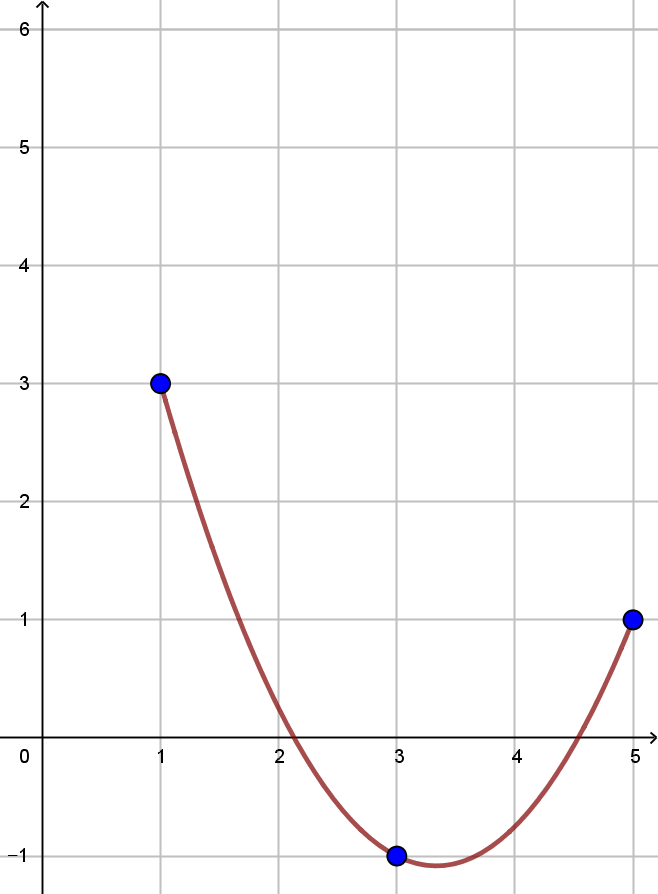
\includegraphics[width=.8\textwidth]{img/2-6-2-2}
\end{center}
\end{minipage}
\end{frame}


\end{document}